% !TeX root = ../main.tex
\section{Homology and Cohomology} % (fold)
\label{sec:homology}

Simplicial complexes not only provide a comprehensive discretization of continuous domains, but are the primary tool for concrete calculations in algebratic topology.
In particular, the study of simplicial homology groups and its dual cohomology groups rely on simplicial complexes in order to study important topological invariants of a discretized space.

% Given a $d$-dimensional simplicial complex $K$ we first induce an orientation on the simplices $\sigma\in K$ by imposing an ordering on its vertex set.
% Two orderings are said to be equivalent if they differ from one another by an even permutation.
% If $\dim(\sigma) > 0$ the orderings of the vertices of $\sigma$ fall into two equivalence classes, each called an \textbf{orientation} of $\sigma$.
% An \textbf{oriented simplex} is a simplex $\sigma$ together with an orientation of $\sigma$.
% We use the notation $[v_0,\ldots, v_p]$ to denote the oriented simplex consisting of vertices $v_0,\ldots, v_p$.

\subsection{Homology}

The following vector spaces may be defined over any field $\F$, however we will assume the field $\F_2$ in order to avoid orienting the simplices in $K$.
Let $C_k(K)$ denote the vector space over some field $\F$ consisting of linear combinations of $k$-simplices in $K$, which form a basis for $C_k(K)$, known as \textbf{$k$-chains}.
These vector spaces are connected by \textbf{boundary maps} $\partial_k:C_k(K)\to C_{k+1}(K)$ which are linear transformations taking basis elements of $C_k(K)$ to the abstract sum of basis $(k+1)$-simplex faces.
The collection of chains and boundary maps forms a sequence of vector spaces known as the \textbf{chain complex} $\C = (C_*,\partial_*)$
\[
    \ldots\xrightarrow{\partial_{k+1}}
    C_k(K)\xrightarrow{\partial_{k}}
    C_{k-1}(K)\xrightarrow{\partial_{k-1}}
    \ldots\xrightarrow{\partial_2}
    C_1(K)\xrightarrow{\partial_{1}}
    C_0(K)\xrightarrow{\partial_0} 0.
\]

An important property of the boundary maps $\partial_k$ is that the composition of subsequent boundary maps is null.
That is, for all $k$
\[ \partial_k\circ\partial_{k-1} = 0. \]
As a result the image of $\partial_{k+1}$, denoted $\im\partial_{k+1} = \{\partial_{k+1}c\mid c\in C_{k+1}(K)$ is a subspace of the kernel, $\ker\partial_k = \{c\in C_k(K)\mid \partial_k c = 0\}$, of $\partial_k$.
A \textbf{$k$-cycle} of $\C$ is a $k$-chain with empty boundary - an element of $\ker\partial_k$.
Two cycles in $\ker\partial_k$ are said to be \textbf{homologous} if they differ by an element of $\im\partial_{k+1}$.
This leads us to the definition of the \textbf{homology groups} of $K$ as quotient vector spaces $H_k(K)$ over $\F$, defined for $k\in\N$ as
\[ H_k(K) := \ker\partial_k/\im\partial_{k+1}.\]

% A $p$-chain is defined as a functions $c$ from the set of oriented $p$-simplices of $K$ to the integers, such that
% \begin{enumerate}
%     \item $c(\sigma) = - c(\sigma')$ if $\sigma$ and $\sigma'$ are opposite orientations of the same simplex
%     \item $c(\sigma) = 0$ for all but finitely many oriented $p$-simplices $\sigma$.
% \end{enumerate}
% We add $p$-chains by adding their values.
% The resulting \textbf{group of (oriented) $p$-chains} of $K$ is denoted $C_p(K)$ for $p = 0,\ldots, d$.
%
% We now define a homomorphism
% \[ \partial_p: C_p(K)\to C_{p-1}(K) \]
% called the \textbf{boundary operator}.
% For an oriented $p$-simplex with $p > 0$ it is defined
% \[ \partial_p\sigma = \partial_p[v_0,\ldots, v_p] = \sum_{i=1}^p (-1)^i [v_0,\ldots,\hat{v_i},\ldots v_p] \]
% where $\hat{v_i}$ indicates that the vertex $v_i$ is to be deleted from the array.
%
% There are two important groups which arise from the boundary operator on a chain group.
% The group of \textbf{$p$-cycles}, denoted $Z_p(K)$ is defined as the kernel of $\partial_p:C_p(K)\to C_{p-1}(K)$ - that is, the collection of $p$-chains $c\in C_p(K)$ such that $\partial_p(c) = 0$.
% The group of \textbf{$p$-boundaries}, denoted $B_p(K)$, is defined as the image of $\partial_{p+1}:C_{p+1}(K)\to C_p(K)$.
% An important property of the boundary operater is that $\partial_{p-1}\circ\partial_p = 0$ for all $p$, implying that each boundary of a $p+1$ chain must be a $p$-cycle, and therefore $B_p(k)\subset Z_p(K)$.
% We may now define the \textbf{$p$th homology group} of $K$ as the quotient group
% \[ H_p(K) := Z_p(K)/B_p(K). \]

\subsection{Cohomology}

A \textbf{cochain complex} is a sequence $\C = (C^*, \delta_*)$ of $\R$-modules $C^k$ consisting of \textbf{cochains} and module homomorphisms known as \textbf{coboundary maps} $\delta_k:C^k\to C^{k+1}$.
As in homology we have the property that $\delta_{k+1}\circ\delta_k = 0$ for all $k$, leading to a familiar definition of the \textbf{cohomology} of $\C$
\[ H^k(\C) = \ker\delta_k/\im\delta_{k-1}.\]
The equivalence classes of $H^k(\C)$ consist of \textbf{$k$-cocycles}: elements of $\ker\delta_k$ that differ by a \textbf{$k$-coboundary} in $\im\partial_{k-1}$.
Such cocycles are said to be \textbf{cohomologous} if they belong to the same equivalence class in $H^k(\C)$.

The simplest construction of a cochain complex is to dualize a chain complex.
For a simplicial complex $K$ with chain complex $(C_*,\partial_*)$ define $C^k(K)$ to be the module of homomorphisms $\psi:C_k\to\R$.
The coboundary maps $\delta_k$ are defined for cochains $\psi:C_k\to\R$ and $k$-simplices $\sigma\in K$ as
\[\delta_k\psi(\sigma) = \psi(\partial_k\sigma).\]

% The cohomology groups of a simplicial complex is dual to the homology groups, and provides a much richer algebraic structure.
% For abelian groups $A, G$ we define the \textbf{Hom functor} $\Hom(A, B)$ as the group of homomorphisms from $A$ into $G$, where the addition of two homomorphisms is simply the addition of their values in $G$.
% Let $K$ be a simplicial complex and $G$ be an abelian group.
% The group of \textbf{$p$-dimensional cochains} of a simplicial complex $K$ is the group
% \[ C^p(K; G) := \Hom(C_p(K), G). \]
% That is, each $p$-cochain is a homeomorphism from a chain $c\in C_p(K)$ to the abelian group $G$.
% The \textbf{coboundary operator} $\delta$ is defined to be the dual of the boundary operator $\partial_{p+1}: C_{p+1}(K)\to C_p(K)$:
% \[\delta_p : C^p(K; G)\to C^{p+1}(K; G). \]
% The \textbf{cohomology groups} are defined in the same way as the homology groups.
% Letting $Z^p(K; G)$ denote the kernel of $\delta_p$ and $B^p(K; G)$ as the image of $\delta_{p-1}$ we have
% \[ H^p(K; G) = Z^p(K; G)/B^p(K; G).\]
% When the group $G$ is the integers $\Z$ we will write the cohomology group $H^p(K;\Z)$ as $H^p(K)$.

\subsection{Relative Homology and Cohomology}

\subsection{Representative Cycles and Cocycles}

We can find a basis for each homology group $H_p(K)$ and cohomology group $H^p(K)$ consisting of $p$-cycles and $p$-cocycles, respectively.
In general, $p$-cycles represent $p$-dimensional holes in the simplicial complex $K$, where $p$-cocycles can be understood as ``blocking chains.''

\begin{figure}[htbp]
\centering
    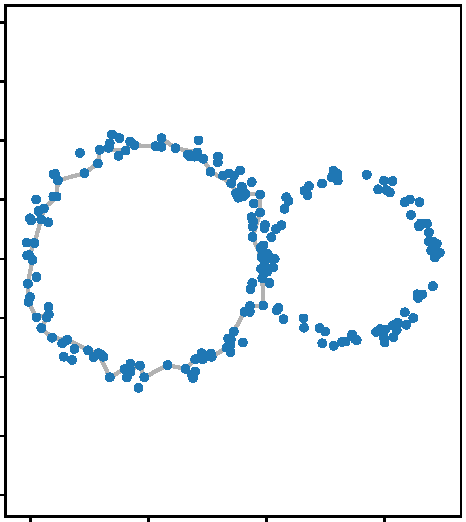
\includegraphics[scale=0.66]{figures/homology_cycle1.pdf}
    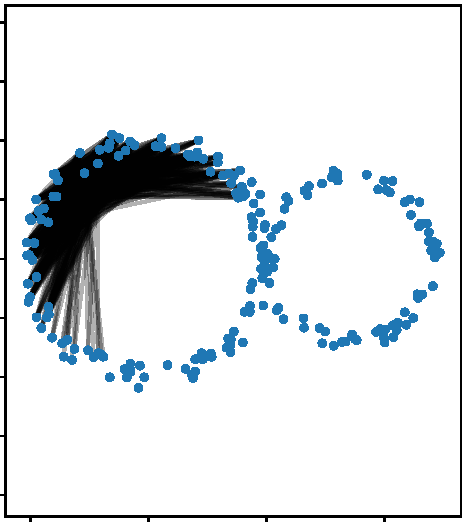
\includegraphics[scale=0.66]{figures/cohomology_cocycle1.pdf}
    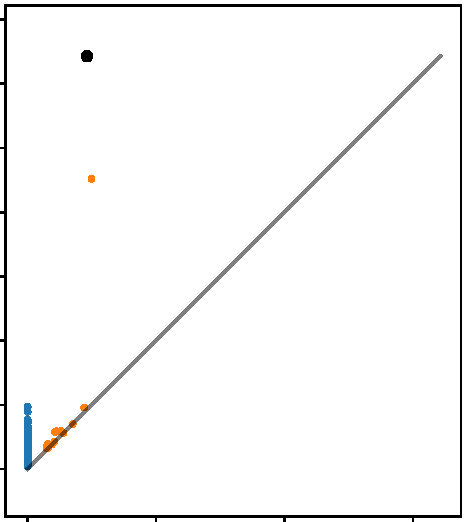
\includegraphics[scale=0.66]{figures/circular_dgm1.pdf}
     \caption{}
     \label{fig:dgm1}
 \end{figure}

 \begin{figure}[htbp]
 \centering
     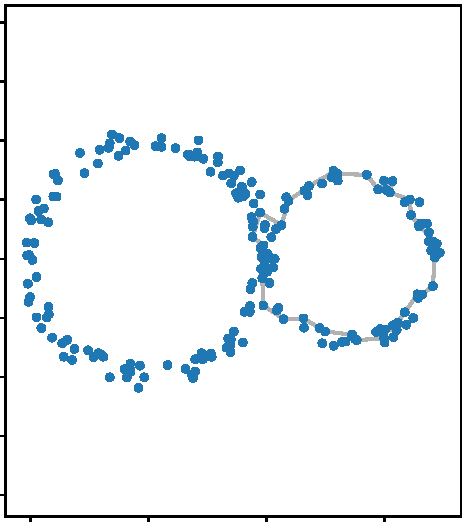
\includegraphics[scale=0.66]{figures/homology_cycle2.pdf}
     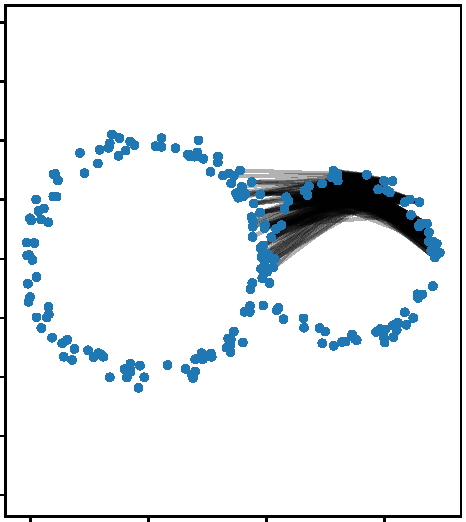
\includegraphics[scale=0.66]{figures/cohomology_cocycle2.pdf}
     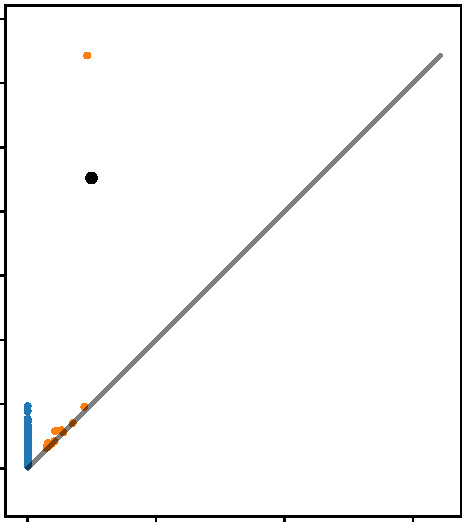
\includegraphics[scale=0.66]{figures/circular_dgm2.pdf}
      \caption{}
      \label{fig:dgm2}
  \end{figure}

\subsection{Persistent Homology and Cohomology}

% section homology (end)
